\chapter{Работа с очередями FIFO}

\emph{Интерфес FIFO. Асинхронных режим. Режимы работы FIFO: Standard и First Word Fall Through. Интерфейс AXI Stream.}

\section{Содержание главы}

Основной литературой по FIFO является PG057. Требуется:
\begin{itemize}
\item описать всю последовательность действий по созданию и кастомизации ядра FIFO, а также включению его в код на VHDL, сделав при этом упор на интерфейс \emph{Native} и на интерфейс \emph{AXI4-Stream} (про интерфейс AXI4 Memory Mapped достаточно упомянуть);
\item написать testbench для ядра FIFO, чтобы показать его функциональность (т.е. то, как ядро работает), привести пример временных форм сигналов из симулятора;
\item описать принцип работы FIFO (описать два указателя~-- на начало и конец очереди в памяти, когда и как они увеличиваются и т.д.);
\item написать, отладить и описать VHDL-код усредняющего FIFO. Обязателен testbench.
\end{itemize}

\section{Оформление}

Очень хорошее и краткое введение в LaTeX можно найти в книге Столярова (\href{url}{http://www.stolyarov.info/books/latex3days/}).

\section{Заголовок 1-го уровня}
\subsection{Заголовок 2-го уровня}
\subsubsection{Заголовок 3-го уровня}

Текст. Текст. Текст. \emph{Текст курсивом.} Поставить тире~-- вот так. Текст в "<кавычках">.

Чтобы сделать новый абзац, нужно пропустить строку.

Пример кода:

\begin{Code}
\begin{lstlisting}
library IEEE;
use IEEE.STD_LOGIC_1164.ALL;

entity Latch is
    port ( C : in  STD_LOGIC;
           D : in  STD_LOGIC;
           Q : out STD_LOGIC);
end Latch;

architecture Behavioral of Latch is
    signal q_tmp : std_logic := '0';
begin
    latch_process: process (C, D)
    begin
        if (C = '1') then
            q_tmp <= D;
        end if;
    end process;
    Q <= q_tmp;
end Behavioral;
\end{lstlisting}
\end{Code}

Пример кода в строке: \lstinline?С = 1?. Или вот так: \lstinline?S(7 downto 1) <= S(6 downto 0);?. Здесь код помещен между знаками вопроса.

Пример нумерованного списка:

\begin{enumerate}
\item Пункт 1.
\item Пункт 2.
\item Пункт 3.
\end{enumerate}

Пример ненумерованного списка:

\begin{itemize}
\item Пункт 1.
\item Пункт 2.
\item Пункт 3.
\end{itemize}

Вот так оформляется таблица с тремя колонками:

\begin{table}[h]
\centering
\begin{tabular}{|c|c|c|}
\hline
input               & \multicolumn{2}{c|}{output} \\ \hline
r                   & code        & active         \\ \hline
\texttt{1{-}{-}{-}} & \texttt{11} & \texttt{1}     \\
\texttt{01{-}{-}}   & \texttt{10} & \texttt{1}     \\
\texttt{001-}       & \texttt{01} & \texttt{1}     \\
\texttt{0001}       & \texttt{00} & \texttt{1}     \\
\texttt{0000}       & \texttt{00} & \texttt{0}     \\
\hline
\end{tabular}
\end{table}

Рисование осуществляется с помощью пакета 'TikZ':

\begin{figure}[ht]
\centering
\begin{tikzpicture}[>=latex']
\tikzstyle{arith_op} = [draw, fill=blue!20, circle, minimum size=2em]

% inputs
\node at (0,4) (input_a) {\texttt{a}};
\node at (0,3) (input_b) {\texttt{b}};
\node at (0,1) (input_c) {\texttt{c}};
\node at (0,0) (input_1) {\texttt{1}};

% operations
\node[arith_op] at (1,3) (block_plus_1) {$+$};
\node[arith_op] at (1,1) (block_plus_2) {$+$};
\node[arith_op] at (2,2) (block_minus) {$-$};

% connections
\draw[->] (input_a) -- (1,4) -- node {} (block_plus_1);
\draw[->] (input_b) -- node {} (block_plus_1);
\draw[->] (input_c) -- node {} (block_plus_2);
\draw[->] (input_1) -- (1,0) -- node {} (block_plus_2);
\draw[->] (block_plus_1) -- (2,3) -- node {} (block_minus);
\draw[->] (block_plus_2) -- (2,1) -- node {} (block_minus);
\draw[->] (block_minus) -- (3,2);
\end{tikzpicture}
\caption{Оптимизированная комбинационная схема.}
\label{label_fig_1}
\end{figure}

Ссылка на рисунок делается по \emph{label} вот так: \ref{label_fig_1}.

Вставка скриншотов программ (PNG) возможна следующим образом (файл изображения находится в папке с кодом):

\begin{figure}[h]
\centering
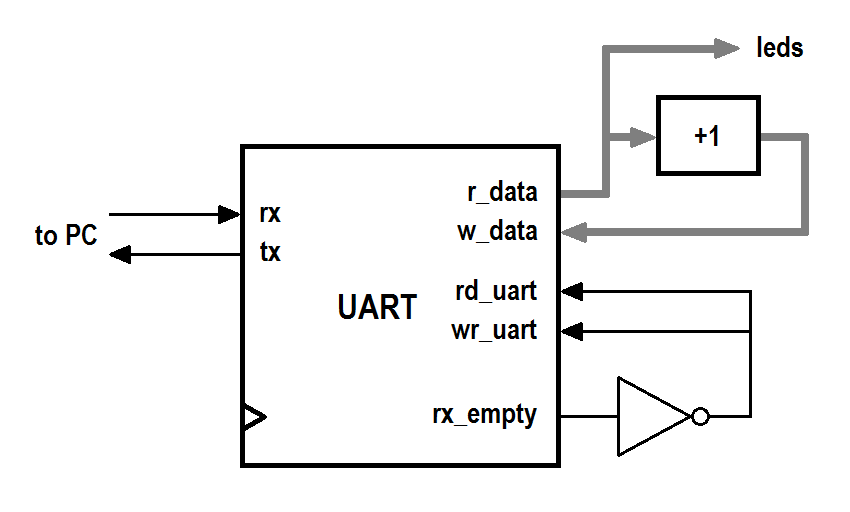
\includegraphics[width=0.6\textwidth]{test_fig}
\caption{Некий рисунок}
\label{test_fig_label}
\end{figure}